
\documentclass[sigplan,review,screen,anonymous]{acmart}
\usepackage[utf8]{inputenc}
\usepackage{mathpartir}

\setcopyright{none}
\definecolor{dkgreen}{HTML}{006329}
\newcommand{\comm}[3]{\textcolor{#1}{[#2: #3]}}
\newcommand{\jwc}[1]{\comm{dkgreen}{JWC}{#1}}

\RequirePackage{listings}
\RequirePackage{xcolor}
\RequirePackage{fvextra}


\colorlet{DFYgreen}{green!40!black}
\colorlet{DFYviolet}{violet}
\colorlet{DFYblue}{blue!50!black}
\colorlet{DFYorange}{orange!70!black}
\colorlet{DFYred}{red!50!black}
\colorlet{DFYgray}{black!70!white}
\colorlet{DFYteal}{teal!80!black}


\RequirePackage{xstring}
\RequirePackage{pgffor}
\RequirePackage{xparse}
\RequirePackage{etoolbox}
\RequirePackage{expl3}

%C
\colorlet{DFYLcommentColor}{DFYgreen}
\colorlet{DFYLnumberColor}{blue}
\colorlet{DFYLKWColor}{DFYblue}
\colorlet{DFYLKW2Color}{DFYgreen}
\colorlet{DFYLstringColor}{DFYred}
\colorlet{DFYLoperatorColor}{DFYred}
\colorlet{DFYLmiscKWColor}{DFYteal}
\colorlet{DFYLcheckerColor}{DFYteal}
%
\makeatletter


% Patch line number key to call line background macro
\lst@Key{numbers}{none}{%
	\def\lst@PlaceNumber{\lst@linebgrd}%
	\lstKV@SwitchCases{#1}%
	{none:\\%
		left:\def\lst@PlaceNumber{\llap{\normalfont
				\lst@numberstyle{\thelstnumber}\kern\lst@numbersep}\lst@linebgrd}\\%
		right:\def\lst@PlaceNumber{\rlap{\normalfont
				\kern\linewidth \kern\lst@numbersep
				\lst@numberstyle{\thelstnumber}}\lst@linebgrd}%
	}{\PackageError{Listings}{Numbers #1 unknown}\@ehc}}

% New keys
\lst@Key{linebackgroundcolor}{}{%
	\def\lst@linebgrdcolor{#1}%
}
\lst@Key{linebackgroundsep}{0pt}{%
	\def\lst@linebgrdsep{#1}%
}
\lst@Key{linebackgroundwidth}{\linewidth}{%
	\def\lst@linebgrdwidth{#1}%
}
\lst@Key{linebackgroundheight}{\ht\strutbox}{%
	\def\lst@linebgrdheight{#1}%
}
\lst@Key{linebackgrounddepth}{\dp\strutbox}{%
	\def\lst@linebgrddepth{#1}%
}
\lst@Key{linebackgroundcmd}{\color@block}{%
	\def\lst@linebgrdcmd{#1}%
}

% Line Background macro
\newcommand{\lst@linebgrd}{%
	\ifx\lst@linebgrdcolor\empty\else
	\rlap{%
		\lst@basicstyle
		\color{-.}% By default use the opposite (`-`) of the current color (`.`) as background
		\lst@linebgrdcolor{%
			\kern-\dimexpr\lst@linebgrdsep\relax%
			\lst@linebgrdcmd{\lst@linebgrdwidth}{\lst@linebgrdheight}{\lst@linebgrddepth}%
		}%
	}%
	\fi
}

\newcommand\storefirst{}
\newcommand\btLstHL[1]{\renewcommand\storefirst{#1}\btLstHLi}

\newcommand{\btLstHLi}[1][\storefirst]{%
	\ifnum\value{lstnumber}<\storefirst%
	\else%
	\ifnum\value{lstnumber}>#1%
	\else%
	\color{HLColor}%
	\fi%
	\fi%
}%

\lst@Key{DFYLnumberstyle}{}{\def\lst@DFYLnumberstyle{#1}}
\lst@Key{formatidstyle}{}{\def\lst@formatidstyle{#1}}
\lst@Key{checkerstyle}{}{\def\lst@checkerstyle{#1}}

\lst@Key{operators}{}{%
	\let\lst@operators\@empty
	\lst@for{#1}\do{%
		\lst@MakeActive{##1}%
		\lst@lExtend\lst@operators{%
			\expandafter\lst@CArg\lst@temp\relax\lst@CDef
			{}\lst@PrintOperator\@empty}}}
\lst@AddToHook{SelectCharTable}{\lst@operators}

\gdef\lst@PrintOperator#1\@empty{%
	\lst@XPrintToken
	\begingroup
	\lst@modetrue \lsthk@TextStyle
	\let\lst@ProcessDigit\lst@ProcessLetter
	\let\lst@ProcessOther\lst@ProcessLetter
	\lst@lettertrue
	#1%
	\lst@SaveToken
	\endgroup
	\lst@RestoreToken
	\global\let\lst@savedcurrstyle\lst@currstyle
	\ifnum\lst@mode=\the\lst@Pmode
	\let\lst@currstyle\lst@gkeywords@sty
	\fi
	\lst@Output
	\let\lst@currstyle\lst@savedcurrstyle}




% ``state variables''
\newif\ifinstring
\def\instringtrue{\global\let\ifinstring\iftrue}
\def\instringfalse{\global\let\ifinstring\iffalse}
\newif\ifinidentifier
\def\inidentifiertrue{\global\let\ifinidentifier\iftrue}
\def\inidentifierfalse{\global\let\ifinidentifier\iffalse}
\newif\ifinbrace
\def\inbracetrue{\global\let\ifinbrace\iftrue}
\def\inbracefalse{\global\let\ifinbrace\iffalse}
\newif\ifincomment
\def\incommenttrue{\global\let\ifincomment\iftrue}
\def\incommentfalse{\global\let\ifincomment\iffalse}
\newif\ifintick
\def\inticktrue{\global\let\ifintick\iftrue}
\def\intickfalse{\global\let\ifintick\iffalse}
\newif\ifDFYLparsenumbers
\lst@AddToHook{Output}{\@DFYLlcaddedToOutput}
\lst@AddToHook{EndGroup}{\inbracefalse\instringfalse\incommentfalse\intickfalse}
\lst@AddToHook{AfterBeginComment}{\incommenttrue}
% local variables
\newif\ifidentifierStartsByDigit@
\newif\ifidentifierStartsByPercent@
\newif\ifidentifierStartsByColumn@
\newif\ifidentifierStartsByColumn@
\def\splitfirstchar#1{\@splitfirstchar#1\@nil}
\def\@splitfirstchar#1#2\@nil{\gdef\@testChar{#1}}
\def\@testChar%
{%
	\ifDFYLparsenumbers
	% copy the first token in \the\lst@token to \@testChar
	\expandafter\splitfirstchar\expandafter{\the\lst@token}%
	\ifidentifierStartsByPercent@%
	\ifinstring%
	\def\lst@thestyle{\lst@formatidstyle}%
	\fi%
	\fi%
	%checker stuff
	\ifinbrace%
	\ifinstring%
	\def\lst@thestyle{\lst@stringstyle}%
	\else%
%	\ifidentifierStartsByColumn@%
	\def\lst@thestyle{\lst@checkerstyle}%
%	\else%
%	\fi%
	\fi%
	\else%
	\fi	%	
	% reset switch
	\identifierStartsByDigit@false%
	\identifierStartsByPercent@false%
	\identifierStartsByColumn@false%
	% equality test
	\IfInteger{\@testChar}{\identifierStartsByDigit@true}{}%
	\IfStrEq{\@testChar}{\%}{\identifierStartsByPercent@true}{}%
	\IfStrEq{\@testChar}{:}{\identifierStartsByColumn@true}{}%
	% processing the tests
	% numbers processing
	\ifidentifierStartsByDigit@%
	\ifnum\lst@mode=\the\lst@Pmode%
	\let\lst@thestyle=\lst@DFYLnumberstyle%
	\fi
	\fi
	% format string identifiers
	\ifidentifierStartsByPercent@%
	\ifinstring
	\def\lst@thestyle{\lst@formatidstyle}%
	\else
	\identifierStartsByPercent@false%
	\fi
	\fi
	\fi
}
\let\@DFYLlcaddedToOutput\@testChar


\makeatother


\lstdefinelanguage
{Dafny}
{
	alsoletter={0123456789?_'},
	showstringspaces = false,
	morestring = [s][\instringtrue\color{DFYLstringColor}]{"}{"},
	moredelim = *[s][\inbracetrue]{\{:}{\}},
	morecomment=[s]{/*}{*/},
	morecomment=[l]//,
	operators={&,|,:,=,+,!,-,>,<,\%},
	morekeywords=[0]{bool, char, int, int32, int64 iset, map, multiset, 
		nat, null, real, seq, set,
		string, Ref, usize, String,
		array, array1, array2, array3, array4, %arrayToken up to 4
		},
	morekeywords = [1]{++,+=,&&,!=,>=,<=,=,+,||,\%},
	morekeywords=[2]{abstract , as , assert , assume , break ,
		calc , case , class , codatatype , colemma ,
		constructor , copredicate , datatype , decreases ,
		default , else , ensures , exists , extends , false ,
		forall , free , fresh , function , ghost , if , imap , import ,
		in , include , inductive , invariant , iterator , label ,
		lemma , match , method , modifies , modify ,
		module , new , newtype , object ,
		old , opened , predicate , print , protected ,
		reads , refines , requires , return , returns , 
		static , then , this , trait , true , type ,
		var , where , while , yield , yields, opaque, reveal,
	    export, provides, reveals, by, for},  %additional keywords
    	%list taken from dafny reference manual, moved types to KW0
    morekeywords=[3]{Exception, U, Result, List, T, Box, 
    Option, RefL, MRef, MRefL,ArrayList,  
    int32, A, Iterator}, %types specific to this paper
    morekeywords = [4]{'l},
    keywordstyle=[3]\bfseries\color{DFYLKWColor},
	keywordstyle=[0]\bfseries\color{DFYLKWColor},
	keywordstyle=[2]\bfseries\color{DFYLKW2Color},
	commentstyle=\color{DFYLcommentColor},
	DFYLnumberstyle=\color{DFYLnumberColor},
	stringstyle=\color{DFYLstringColor},
	formatidstyle=\color{DFYLnumberColor},
	checkerstyle=\color{DFYLcheckerColor},
	keywordstyle=[1]\color{DFYLoperatorColor},
	keywordstyle=[4]\color{DFYLstringColor},
}

\lstnewenvironment{dafny}[1][]{
	\lstset{ %
		basicstyle=\ttfamily,
		breakatwhitespace=true,
		breaklines=true,
		extendedchars=true,
		keepspaces=true,
		showspaces=false,
		showstringspaces=false,
		showtabs=false,
		tabsize=2,
		language=Dafny,
		#1
	}\DFYLparsenumberstrue
}{\DFYLparsenumbersfalse}

\lstdefinestyle{dafnyS}
{
	language=Dafny,columns=fixed,
	basicstyle={\ttfamily},
}



% ===== Authors =====

\author{Joseph W. Cutler}
\email{jwc@seas.upenn.edu}
\orcid{0000-0001-9399-9308} % chktex 8
\affiliation{%
  \institution{University of Pennsylvania}
  \city{Philadelphia}
  \state{Pennsylvania}
  \country{USA}
}

\author{Emina Torlak}
\email{emina@cs.washington.edu}
\orcid{} % chktex 8
\affiliation{%
  \institution{Amazon Web Services}
  \city{Seattle}
  \state{Washington}
  \country{USA}
}

\author{Michael Hicks}
\email{mwh@cs.umd.edu}
\orcid{} % chktex 8
\affiliation{%
  \institution{Amazon Web Services}
  \city{Arlington}
  \state{Virginia}
  \country{USA}
}

\renewcommand{\shortauthors}{Cutler et al.}

% Draft title
\title{Improving the Stability of Type Soundness Proofs in Dafny}

\begin{abstract}
  In this extended abstract, we present a systematic technique for
  structuring type soundness proofs in Dafny to improve proof stability. As a case
  study, we apply the method to proving type soundness for a small expression
  language, and demonstrate empirically how it improves resource usage metrics
  known to correlate with stability. Our method can scale to realistic proofs,
  as demonstrated by its use in the type soundness proof of the Cedar Policy
  Language.
\end{abstract}

\keywords{}

\begin{document}
\maketitle

\section{Introduction}

\begin{itemize}
    \item Explain the problem statement and setup:
    \item \begin{itemize}
      \item you've got a langauge, deeply embedded in dafny.
      \item This means that you have some big-step semantics for the language, implemented by a definitional interpreter which returns either a value, or an error. (show generic)
      \item You also have a typechecker, written in dafny: a boolean function which checks if a program has some type.  (show generic)
            This ideally implements some particular type system (presented declaratively, with rules). This usually works where there's one rule for each syntactic form, adn so the function pattern matches on the syntax, and makes recursive calls to check or infer the types of the premises.
      \item You want to show a soundness theorem, which states that well-typed programs are safe: either the program successfully evaluates to a value of the correct type, or it encounters one of some allowable class of errors. (show example, with examples of safety -- errors or no errors)
    \end{itemize}

    \item How do you do the proof?
    \begin{itemize}
      \item Proofs of type soundness on paper are by induction on typing derivations
      \item In dafny, this looks like pattern matching on the term, and making recursive calls for the IH. (show this scaffold)
      \item These proofs grow linearly with the size of the language: more cases for more kinds of expressions.
    \end{itemize}

    \item It's important that this proof be \emph{stable}. 
    \begin{itemize}
      \item Unlike mechanized metatheory developments in tools backed by a type-theoretic proof checker, Dafny's SMT-backed verification
      can be \emph{unstable}: the result of verifying the type soundness theorem
      can change, seemingly at random.

      \item Proof instability is empirically known to correlate with both (a) proof resource usage, and (b) proof resource usage \emph{variance}.
      Proofs which use a lot of resoruces are likely to be unstable, as are proofs which may vary greatly in their resource usage between runs.
    \end{itemize}

    \item The problem:
    \begin{itemize}
      \item Unfortunately, traditional direct-style proofs of type soundness are very unstable in dafny, and do not scale to realistic-scale langauges.
      \item (Color on the whack-a-mole issue) 
    \end{itemize}

    \item Contributions: 
    \begin{itemize}
      \item Demonstrate a technique for making mechanized metatheory proofs more stable (Section~\ref{sec:sts}) by axiomatizing \jwc{word} the evaluator and type checker.
      \item Evaluate the technique by comparing empirical metrics of proof stability against other methods of structuring the proof (Section~\ref{sec:eval}).
    \end{itemize}

    \item In Section~\ref{sec:discussion}, we'll discuss details of how the technique might apply in different situations, as well as how it was developed and deployed to build the type soundness proof for the cedar language.

    \jwc{Mention that this is used in Cedar, and cite the open-source development}

    \jwc{Make sure to namecheck the blog post}
    
\end{itemize}

\section{Stable Type Soundness Proofs}
\label{sec:sts}

\jwc{Build into this better.}
For a running example, let's consider the first-order expression language we
use for our evaluation in Section~\ref{sec:eval}.  The language has
types for integers, booleans, and records, all given as the Dafny type
\texttt{Ty}.  For terms, we have variables (represented as strings, since the
langauge has no binders), addition, subtraction, division, and, or,
conditionals, and record expressions and projections. These are all represented
by a Dafny ADT \texttt{Term}, which has a variant for each syntactic form.
To demonstrate how the language works, and how our technique applies, we focus
on just the behavior of the addition operation.

The language's semantics is implemented by a program \texttt{eval(env,e)} which takes an environment \texttt{type
Env = map<string,Val>} mapping variables to their values and a term, and returns
either (a) the value the term evaluates to, or (b) an evaluation error, which can be a
division by zero error or a runtime type error.

The function header for the \texttt{eval} function is shown in Figure~\ref{fig:eval}.
The function \texttt{evalInt} is a helper that calls \texttt{eval}, and then pattern matches on the result,
returning \texttt{n} if it was \texttt{IntVal(n)}, and throwing a runtime type error otherwise.

\begin{figure}
\begin{dafny}
function eval(env : Env, e : Term) : Result<Val,EvErr>
{
  match e {
    ...
    case Add(e1,e2) =>
      var n1 :- evalInt(env,e1);
      var n2 :- evalInt(env,e2);
      Ok(IntVal(n1 + n2))
  }
}
  \end{dafny}
  \caption{The \texttt{eval} function, with the case for \texttt{Add}}
  \label{fig:eval}
\end{figure}


Terms are typed in a context \texttt{type Ctx = map<string,Ty>} mapping variables to their types,
with a typechecking implemented by a program \texttt{check(ctx,e,t)} which calls an inference function \texttt{infer}, and then checks if the result is equal to \texttt{t}.
Code for \texttt{check} and the \texttt{Add} case for \texttt{infer} are shown in Figure~\ref{fig:infer}, where
\texttt{inferIntTy} calls \texttt{infer}, and throws a type error if the result
is anything but \texttt{IntTy}.

\begin{figure}
\begin{dafny}
function check(ctx : Ctx, e : Term, t : Ty) : Result<(),TckErr> {
  var t' :- infer(ctx,e);
  if t == t' then Ok(()) else Err(TckErr)
}

function infer(ctx : Ctx, e : Term) : Result<Ty,TckErr> {
  match e {
    ...
    case Add(e1,e2) =>
      var _ :- inferIntTy(ctx,e1);
      var _ :- inferIntTy(ctx,e2);
      Ok(IntTy)
    }
  }
\end{dafny}
\caption{The \texttt{check} and \texttt{infer} functions, with the case for \texttt{Add}}
\label{fig:eval}
\end{figure}



\subsection*{A First Cut}

For this language, type soundness means the following. If \texttt{e} checks against \texttt{t} in context
\texttt{ctx} and the environment
\texttt{env} agrees with the context \texttt{ctx},
then \texttt{e} either evaluates under the environment \texttt{env} to a value of type \texttt{t}, or it results
in a division by zero error (but not a runtime type error). 
This lemma is encoded in dafny as the \texttt{sound} lemma in Figure~\ref{fig:sound},
along with auxiliary definitions: \texttt{envHasCtx} is the predicate saying that the environment agrees with the context,
and \texttt{isSafe(env,e,t)} encodes the conclusion of the theorem.

\begin{figure}
\begin{dafny}
lemma sound(env : Env, ctx : Ctx, e : term, t : Ty)
  requires envHasCtx(env,ctx)
  requires check(ctx,e,t).Some?
  ensures isSafe(env,e,t)
{
  match e {
    ...
    case Add(e1,e2) =>
      sound(env,ctx,e1,IntTy);
      sound(env,ctx,e2,IntTy);
  }
}

predicate envHasCtx(env : Env, ctx : Ctx) {
  forall x :: x in ctx ==>
    x in env &&
    valHasType(env[x],ctx[x])
}

predicate isSafe(env : Env, e  : Term, t : Ty){
  (eval(env,e).Ok? && valHasType(eval(env,e).value,t))
  ||
  (eval(env,e).Err? && eval(env,e).error == DivByZero)
}
\end{dafny}

  \caption{The \texttt{sound} lemma with the case for \texttt{Add}, and auxiliary definitions}
\end{figure}


To prove the \texttt{sound} lemma, we induct on the term \texttt{e}.
The case of \texttt{sound} for \texttt{Add(e1,e2)} is illustrative.
We make two recursive calls to the lemma to introduce the inductive hypotheses,
and the solver takes care of the rest. 

The reasoning that the solver takes care of under the hood is somewhat involved.
Getting from the assumption \texttt{check(ctx,Add(e1,e2),t).Some?} to
the IH preconditions \texttt{check(ctx,e1,IntTy).Some?} and
\texttt{check(ctx,e2,IntTy).Some?} requires reasoning about the (potentially complex) code for
\texttt{check} and \texttt{infer}. Similarly, getting from the IH results \texttt{isSafe(env,e1,IntTy)} and
\texttt{isSafe(env,e2,IntTy)} to the conclusion
\texttt{isSafe(env,Add(e1,e2),t)} requires reasoning through the code for \texttt{eval} to determine the possible
ways \texttt{Add(e1,e2)} evaluates when \texttt{e1} and \texttt{e2} might either evaluate to values or
raise division-by-zero errors.

\subsection*{Finding Stability}
\jwc{Fix sectionname}

Unfortunately, as we'll see in Section~\ref{sec:eval}, this proof approach is
not stable. We realized this while attemping to scale this style
of proof up to a realistic language. With enough operations and language
features, the proof resource usage varies wildly between runs,
enough that the verification will fail at random. At its core, this
instability arises from all of the afformentioned unguided reasoning the solver has to do about the
code of the typechecker and evaluator,
to get from the premise of the lemma to the premises of the IH, and then
from the conclusions of the IH to the conclusion of the case.
A patchwork solution is to add guidance in the form of assertions around the
recursive calls, to spell out the intermediate steps more directly.
\jwc{Words, about why this doesn't work in the long run}

A common and more robust solution to dealing with proof instability is to specify
the functions involved in the proof, and then make the functions themselves opaque.
This way, the solver can only interact with the functions though the specification,
cutting down the search space of possible proofs and hence improving stability.
Moreover, if the specifications are written in the form of separate lemmas,
the programmer can control how and when different parts of the function's sepcification
is revealed to the solver.

But which functions to make opaque, and how to specify them?
Inspiration comes from noticing that \texttt{sound} depends only on
facts about the safety predicate \texttt{isSafe}, and not directly
on facts about evaluation. In fact, the only facts it needs about \texttt{isSafe}
are that in every case, the results of the IH calls jointly imply the conclusion.
To illustrate, the addition case for type soundness holds
for \emph{any} safety predicate \texttt{isSafe} --- even an opaque one --- which has the property
that \texttt{isSafe(env,e1,IntTy)} and \texttt{isSafe(env,e2,IntTy)}
together imply \texttt{isSafe(env,Add(e1,e2),IntTy)}.


\begin{figure}
\begin{dafny}
lemma addIsSafe(env : Env, e1 : Expr, e2 : Expr)
  requires isSafe(env,e1,IntTy)
  requires isSafe(env,e2,IntTy)
  ensures isSafe(env,Add(e1,e2),IntTy)
{reveal isSafe(); ...}
\end{dafny}
  \caption{Add Compatibility Lemma}
  \label{fig:add-is-safe}
\end{figure}

This lemma, shown as \texttt{adIsSafe} in Figure~\ref{fig:add-is-safe} is a kind
of ``compatibility lemma'', stating that safe terms can be built from smaller
safe terms.  The upshot from this is that if we make the \texttt{isSafe}
predicate opaque, the \texttt{Add} case of the soundess theorem goes through
with only minor modification, adding a call to \texttt{addIsSafe} after the uses
of IH.

\begin{dafny}
lemma sound(env : Env, ctx : Ctx, e : term, t : Ty)
  requires envHasCtx(env,ctx)
  requires check(ctx,e,t).Some?
  ensures isSafe(env,e,t)
{
  match e {
    ...
    case Add(e1,e2) =>
      sound(env,ctx,e1,IntTy);
      sound(env,ctx,e2,IntTy);
      addIsSafe(env,e1,e2);
  }
}
\end{dafny}

One way of thinking about the \texttt{addIsSafe} lemma is that it says that the
safety predicate \emph{interprets the typing rule} for addition. By by replacing
all instances of the typing judgent in the rule for Addition that the case of \texttt{infer}
for \texttt{Add(e1,e2)} implements, we arrive at the required \texttt{addIsSafe} compatibility lemma:
this is demonstrated in Figure~\ref{fig:tck-to-lemma}.  In short, all that's required for a given safety predicate to hold for every well-typed term is
that it interprets every typing rule in the language. This suggests the following technique:

\begin{figure}
  \begin{mathpar}
  \infer{\texttt{ctx} \vdash \texttt{e1} : \texttt{IntTy} \\ \texttt{ctx} \vdash \texttt{e2} : \texttt{IntTy}}
  {
    \texttt{ctx} \vdash \texttt{Add(e1,e2)} : \texttt{IntTy}
  }
  \\
  \mprset { fraction ={\cdot \cdots \cdot}}
  \infer{\texttt{isSafe(env,e1,IntTy)} \\ \texttt{isSafe(env,e1,IntTy)}}
  {
    \texttt{isSafe(env,Add(e1,e2),IntTy)}
  }
  \end{mathpar}
  \caption{Addition Typing Rule, and the Corresponding Compatibility Lemma}
  \label{fig:tck-to-lemma}
\end{figure}

\begin{enumerate}
  \item Make the safety predicate opaque, preventing the solver from directly reasoning about the interpreter in the type safety proof.
  \item Prove ``safety compatibility lemmas'' for every typing rule, demonstrating that if the safety predicate holds of all the premises, it holds of the conclusion.
  \item Write the type soundness proof, inserting calls to each case's corresponding compatibility lemma, just after the recursive calls to IH.
\end{enumerate}

\subsection*{Going Further with Inversion Lemmas}

Even with this modification, the type soundness proof still requires the solver to
do complex reasoning about the code of the typechecker. To eliminate this unguided
reasoning, we must find a way to specify the typechecker enough to make it opaque,
and have the main soundness proof refer only to the specification lemmas.

Our solution again comes from an analysis of what the solver needs to know about
\texttt{check} in each case. In the \texttt{Add(e1,e2)} case, the solver must
reason from \texttt{check(ctx,Add(e1,e2),t).Ok?} to \texttt{check(ctx,e1,IntTy).Ok?} and
\texttt{check(ctx,e2,IntTy).Ok?} for the preconditions of the IH to hold, essentially
running the code of \texttt{infer} and \texttt{check} in reverse.  This kind of reasoning
corresponds to what's known in the type systems literature as \emph{inversion
principles}: theorems that state that if the a compound syntactic form (like
\texttt{Add(e1,e2)}) is well-typed, then its component forms (here, \texttt{e1}
and \texttt{e2}) are well-typed. Moreover, this inversion lemma, shown in Figure~\ref{fig:add-invert} is slightly stronger, saying that
the type \texttt{t} in question must have been \texttt{IntTy}.


\begin{figure}
\begin{dafny}
  lemma invertAddCheck(ctx : Ctx, e1 : Term, e2 : Term)
  requires invert(ctx,Add(e1,e2),t).Ok?
  ensures check(ctx,e1,IntTy).Ok?
  ensures check(ctx,e2,IntTy).Ok?
  ensures t == IntTy
{ reveal infer(); reveal check(); }
\end{dafny}

  \caption{Inversion Lemma for Addition}
  \label{fig:add-invert}
\end{figure}

This then allows us to make the \texttt{check} and \texttt{infer} functions opaque, and modify
the proof of the soundness theorem once more to add a call to this inversion lemma before the calls to IH.

\begin{dafny}
lemma sound(env : Env, ctx : Ctx, e : term, t : Ty)
  requires envHasCtx(env,ctx)
  requires check(ctx,e,t).Some?
  ensures isSafe(env,e,t)
{
  match e {
    ...
    case Add(e1,e2) =>
      invertAddCheck(ctx,e1,e2);
      sound(env,ctx,e1,IntTy);
      sound(env,ctx,e2,IntTy);
      addIsSafe(env,e1,e2);
  }
}
\end{dafny}

This gives us the final recipe for our technique:

\begin{enumerate}
  \item Make the safety predicate opaque, preventing the solver from directly reasoning about the interpreter in the type safety proof.
  \item Prove safety compatibility lemmas for every typing rule, demonstrating that if the safety predicate holds of all the premises, it holds of the conclusion.
  \item Make the typechecker opaque
  \item Prove inversion lemmas for every typing rule, showing that if the typechecker can compute that the concluson holds, it must also be able to compute that the premises.
  \item Write the type soundness proof, inserting calls to the inversion lemmas before IH calls, and inserting calls to the compatibility lemma after.
\end{enumerate}


% \jwc{This makes the type safety proof completely generic to the implementation
% of the typecheker and evaluator. You can chance the way they're implemented, add
% new cases, do any number of refactors. If you fixup the compatibility and
% iversion lemmas, you're good to go. As we'll see in the next section, it also
% makes the proofs vary way less.}




\section{Evaluation}
\label{sec:eval}
In this section, we demonstrate empirically that our technique as described in Section~\ref{sec:sts}
does yield more stable type soundness proofs. As a quantative proxy for stability, we will measure
the resource usage of our proofs. If a proof is expensive, or its cost varies wildly
between runs, this can be an indicator for future proof instability \jwc{Aaron Tomb, personal communication}.
While resource usage is the most important indicator of future proof instability, we also
base our conclusions on how much verification duration --- the wall-clock time it takes for the solver
to prove the VCs --- varies between runs.

\subsection*{Experimental Setup}
We evaluate five different typecheckers and type soundness proofs for the same
language to compare their proof stability.  The code for these typecheckers, proofs, and the language's evaluator, can be found in
the supplementary materials. The five different typecheckers, as well as the contents of the rest of the files, are described below.
\jwc{Give these better names}

\begin{itemize}
  \item (\texttt{lang.dfy}): The langauge and type definitions, common to all typecheckers and the evaluator.
  \item (\texttt{eval.dfy}): Contains the evaluator for our expressiong language. All of the type soundness proofs are relative to this evaluator.
  \item (\texttt{monadic.dfy}): This is the typechecker and type safety proof described in
  the first part of Section~\ref{sec:sts}.  The typechecker uses one main method
  \texttt{infer} and some helper functions to infer a type for a term, and then checks
  that it's equal to the given type. \jwc{Go back and make this true, in the code}
  \item (\texttt{direct}): This is the same as the typechecker in \texttt{monadic.dfy}, with all of the
  syntactic sugar for \texttt{Result}-binds (\texttt{:-}) unfolded, and all of the helper
  functions inlined. We include this file to measure the degree to which adding
  layers of abstraction hurts proof stability. The proof is essentially the same as the one in \texttt{monadic.dfy}.
  \item (\texttt{bidirectional.dfy}): This typechecker is written in the same style as the typechecker in \texttt{monadic.dfy}. The typing relation that it impelents is slightly different,
        however, including a subtyping rule which implements record width and depth subtyping.
        The type soundness proof changes to include calls to reflexivity and transitivity lemmas about subtyping, which cannot be inferred by the solver.
  \item (\texttt{semantic.dfy} \jwc{fix}):
        This file implements the first half of our technique, making the safety
        property opaque, proving compatability lemmas about the evaluator, and
        calling them in the soundness proof.  The typechecker is identical to
        the one in \texttt{bidirectional.dfy}.
  \item (\texttt{semantic-invert.dfy}): This file implements the full stabilizing technique, adding
  \item (\texttt{std.dfy} and \texttt{util.dfy}): Auxiliary functions and definitions not specific to the language's evaluator or typechecker.
\end{itemize}

We run the experiment by running the built-in \texttt{dafny measure-complexity}
command on the files containing each type soundness proof, with the flags \texttt{--iterations:250 --log-format csv}.
Each invocation of \texttt{measure-complexity} command verifies the file $250$ times, and dumps
the verification results, durations, and resource usages to a CSV file. We then parse and analyze the CSV
file with a python script, which computes the means and standard deviations of verification duration and resource usage for the solver's task of proving correctness
of the VCs in the file's main soundness theorem.
The experiments were run on a 2023 MacBook Pro with an Apple Silicon M2 processor, and 32GB memory, runnning Dafny v4.3.0, and z3 v4.12.1.

\subsection*{Results}
The graph in Figure~\ref{fig:results} shows the mean verification \emph{resource usage} (and standard deviation, with whiskers), over the 250 verifications of each soundness theorem.

% \begin{itemize}
%   \item We look at the mean verification \emph{duration} and \emph{resource usage}
%         over 250 verifications --- lower is better in both cases, meaning that the proof takes less time and is less costly on average.
%   \item Of greater interest is the \emph{variance} of duration and resource usage. A proof which vareis wildly in its verification duration or resource usage
%         is often a precursor to a proof whose outcome varies. \jwc{Cite Aaron Tomb, personal communication} This is shown with whiskers (standard deviations)
% \end{itemize}

\begin{figure}
  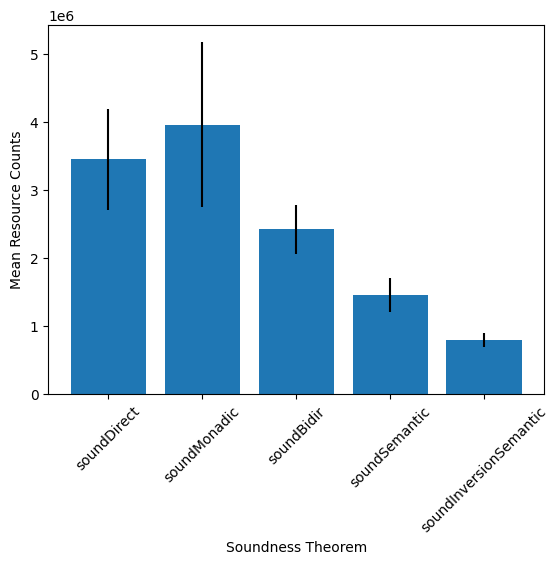
\includegraphics{costgraph.png}
  \caption{Verification Resource Usages}
\end{figure}
\jwc{Graph 1}

The highest cost and highest variance proof in all cases is the soundness proof for the typechecker in \texttt{monadic.dfy}. It strikes an unforuntate balance of being complicated code --- heavy use of monadic bind and lots of helper functions --- with little guidance in the proof.
The typechecker in \texttt{direct.dfy} is slightly cheaper to verify than the one in \texttt{monadic.dfy}, but it still has enormous variance. The cost seems to be lower because of all of the inlined definitions,
meaning that the verifier must reason about fewer functions while proving soundness.
The proof for the typechecker in \texttt{bidirectional.dfy} is cheaper and has lower variance than either of the previous two. This may be because while the bidirectionality increases the complexity of the typechecking algorithm,
this complexity \emph{requires} further guidance to the verifier for it to accept the proof at all, thereby improving stability on the whole.
As expected, the two proofs using the first and second halves of our technique
are by far the best. The soundness theorem using the fully specified typechecker and safety property (\texttt{semantic-invert.dfy})
is the best of all, with negligable variance in resource usage between runs of the verifier.

\section{Discussion}

\subsubsection*{Scaling It Up}
A version of this proof technique was developed for the purposes of mechanizing the proof of type soundness
of the Cedar Policy Language \jwc{cite} \footnote{https://github.com/cedar-policy/cedar-spec/tree/main/cedar-dafny},
and the technique described in this abstract is currently used in the type soundness proof of the language.
Cedar's type system is a great deal more complex than that of our toy langauge, and includes a number of advanced type system features like ocurrence typing \jwc{cite: The Design and Implementation of Typed Scheme} and
singleton types \cite{https://dl.acm.org/doi/10.5555/645867.670933}.

Semantically, Cedar is not \emph{all} that much more complex to model than the
toy language we evaluate for this extended abstract. Like our toy language,
Cedar is terminating and first order.  Although we have not tested it, our
technique should scale to languages with nontermination --- by step-indexing the
evaluator and proving type-safety with failure to converge in $n$ steps being
considered ``safe'' \jwc{cite step-indexing} --- and higher-order functions ---
by applying standard tricks to handle variable binding. \jwc{cite}



\subsubsection*{Manual Effort \& Benefit}
All of this benefit does come at the cost of some of the automation that Dafny
users expect. In taking possible work away from the solver to make the proof
more stable, we are necessarily creating more work for ourselves!  As we saw in
the previous section, the type soundness proofs in the last two cases spell out
many more steps along the way.

For language simpler than the one we evaluate here, the benefit of using this technique decreases. In particular, in languages
where the safety property does not include a disjunction --- safety means that every term evaluates to a value of the right type ---
the benefit shrinks dramatically. The kind of straight-line reasoning required when every term can only evaluate in one way seems to be
much easier for the verifier.

\subsection*{Cost of Compatibility and Inverson Lemmas}
\jwc{Decreases instability, but does require extra lemmas! Because the other proofs dont' have these lemmas broken out, we have no way to empircally measure how they compare to the proofs in the other techniques. That being said, we have anecdotatlly found the compatability and inversion lemmas to be very stable with minimal guidance, both in this development and in Cedar.}

\jwc{The compataiblity and inversion lemmas are small and only require reasoning about either the evaluator or the checker.}


\bibliographystyle{ACM-Reference-Format}
\bibliography{refs}

% \newpage
\include{appendix}

\end{document}